% \lecture{4}{Tue 04 Feb 2020 14:30}{393 Lab 4}

\section{Plots of System response varying $\omega_{0}$, $\zeta$}
The result of varying $\zeta$ is the graph in Figure \ref{fig:varying-zeta}.
\begin{figure}[H]
	\centering
	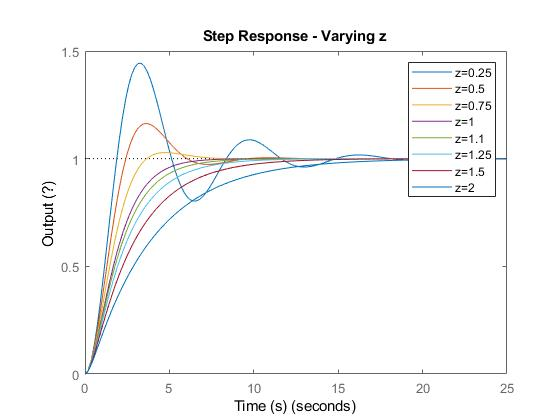
\includegraphics[width=0.8\textwidth]{./figures/lab4_fig1-part4-3-1-z.jpg}
	\caption{A plot of the system response when varying the value of $\zeta$}
	\label{fig:varying-zeta}
\end{figure}
As you can see an increase in $\zeta$ increases the damping of the output, where $\zeta=1$ seems to be close to the critical damping value, $\zeta < 1$ is an underdamped system and $\zeta > 1$ is an overdamped system. 

The result of varying $\omega_{0}$ is seen in Figure \ref{fig:varying-w0}.
\begin{figure}[H]
	\centering
	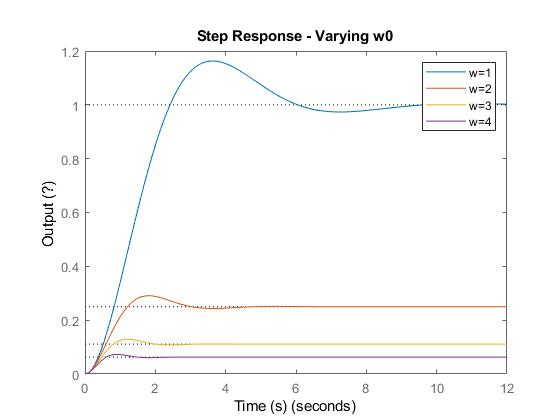
\includegraphics[width=0.8\textwidth]{./figures/lab4_fig2-part4-3-1-w0.jpg}
	\caption{A plot of the system response when varying the value of $\omega _{0}$}
	\label{fig:varying-w0}
\end{figure}
The greater the value of $\omega_{0}$, the smaller the steady-state value of the system. 

\section{Effects of Changing $\alpha$}  %Maxym
For positive values of $\alpha$, the effect of increasing $\alpha$ is the graph in Figure \ref{fig:varying-alpha-positive}.
\begin{figure}[H]
	\centering
	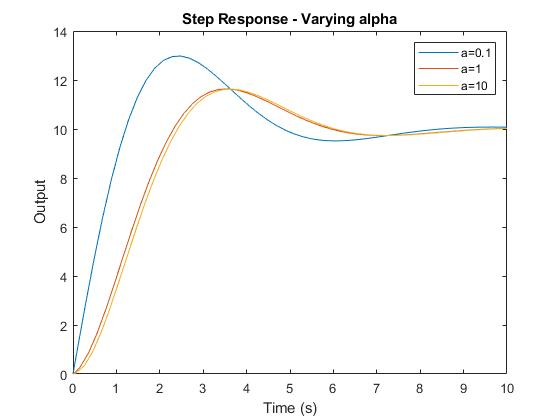
\includegraphics[width=0.8\textwidth]{./figures/lab4_fig3-part4-3-2-positive.jpg}
	\caption{A plot of the system response when varying the positive values of $\alpha$}
	\label{fig:varying-alpha-positive}
\end{figure}
As $\alpha$ increases, the rise time of the system also increases. While there is a large difference between the rise times of $\alpha = 0.1$ and $\alpha = 1$, the difference between $\alpha = 1$ and $\alpha = 10$ is relatively small. Meanwhile, settling time for all positive values of $\alpha$ appear relatively similar with all of the values converging to 10 at approximately 10 seconds. All three positive values of $\alpha$ displayed overshoot with $\alpha = 0.1$ having the largest overshoot while $\alpha =1$ and $\alpha = 10$ had smaller overshoots. Similarly, the peak time of $\alpha = 0.1$ is much shorter than the peak times of $\alpha = 1$ and $\alpha = 10$. The graph shows that $\alpha = 10$ has the longest peak time. 

For negative values of $\alpha$, the effect of increasing $\alpha$ is the graph in Figure \ref{fig:varying-alpha-negative}.
\begin{figure}[H]
	\centering
	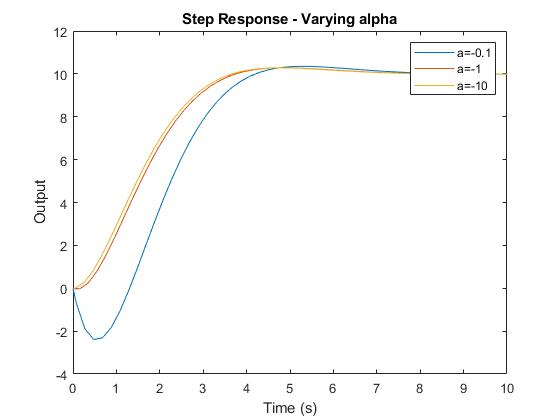
\includegraphics[width=0.8\textwidth]{./figures/lab4_fig4-part4-3-2-negative.jpg}
	\caption{A plot of the system response when varying the negative value of $\alpha$}
	\label{fig:varying-alpha-negative}
\end{figure}
As $\alpha$ increases negatively, the rise time of the system decreases. While there is a large difference between the rise times of $\alpha = -0.1$ and $\alpha = -1$, the difference between $\alpha = -1$ and $\alpha = -10$ is relatively small. Meanwhile, settling time for all negative values of $\alpha$ appear relatively similar with all of the values converging to 10 at just under 10 seconds. All three negative values of $\alpha$ displayed small overshoot with $\alpha = -0.1$ having a slightly larger overshoot than $\alpha =1$ and $\alpha = 10$. The peak time of $\alpha = -0.1$ is slightly longer than the peak times of $\alpha = 1$ and $\alpha = 10$ which had similar peak times.
% End Maxym Section

\section{Non-minimum Phase System}

The plots with and without the additional zero are the same because the impulse response is scaled by $\frac{\omega^{2}_{0}}{\alpha}$. The initial conditions for the system were $y(0)=0$ and $\dot y=\frac{\omega^{2}_{0}}{\alpha}$ so by adding a RHP zero, the system slows down and introduces potential undershoot. However, the scaling of the impulse response counteracts this undershoot. The plots collected can be seen below.

\begin{figure}[H]
              \centering
              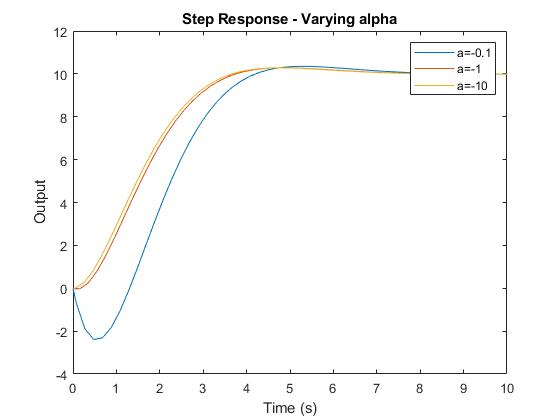
\includegraphics[width=0.8\textwidth]{./figures/lab4_fig4-part4-3-2-negative.jpg}
              \caption{A plot of the system step response when varying the negative values of $\alpha$}
              \label{fig:varying-negative-alpha}
\end{figure}

\begin{figure}[H]
              \centering
              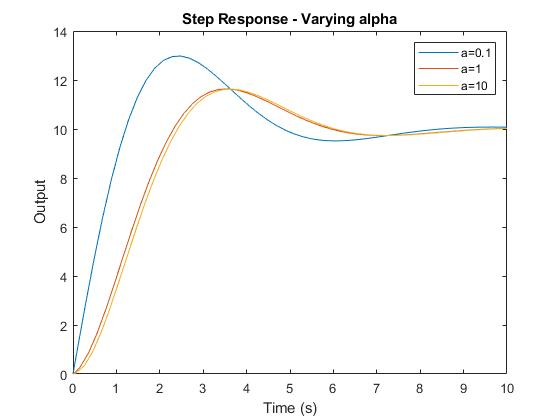
\includegraphics[width=0.8\textwidth]{./figures/lab4_fig3-part4-3-2-positive.jpg}
              \caption{A plot of the system step response when varying the positive values of $\alpha$}
              \label{fig:varying-positive-alpha}
\end{figure}

\begin{figure}[H]
              \centering
              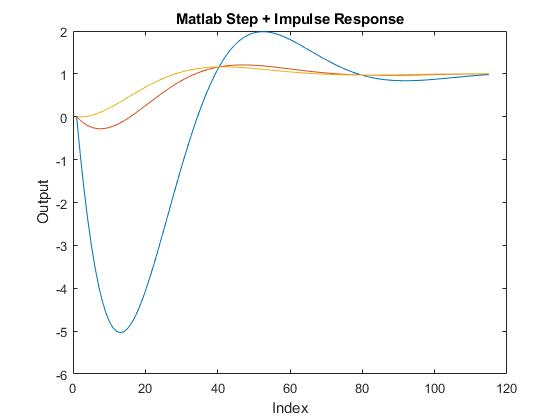
\includegraphics[width=0.8\textwidth]{./figures/lab4_fig6-part4-3-2-matlab-b-negative.jpg}
              \caption{A plot of the system step and impulse response with positive $\alpha$ values and with impulse response scaled by $\frac{\omega^{2}_{0}}{\alpha}$}
              \label{fig:stepimpulse-negative-alpha}
\end{figure}

\begin{figure}[H]
              \centering
              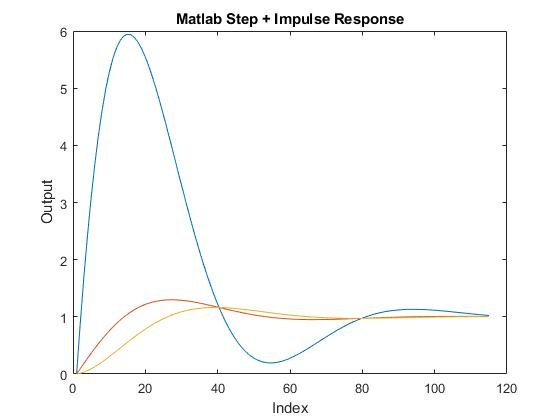
\includegraphics[width=0.8\textwidth]{./figures/lab4_fig6-part4-3-2-matlab-b-positive.jpg}
              \caption{A plot of the system step and impulse response with negative $\alpha$ values and with impulse response scaled by $\frac{\omega^{2}_{0}}{\alpha}$}
              \label{fig:stepimpulse-positive-alpha}
\end{figure}


\section{System Type Section} %Alex 

\begin{table}[h]
\begin{tabular}{|l|l|l|l|l|}
System & \begin{tabular}[c]{@{}l@{}}Response to \\ Constant Input\end{tabular}                    & \begin{tabular}[c]{@{}l@{}}Response to \\ Linear Input\end{tabular}                      & \begin{tabular}[c]{@{}l@{}}Response to \\ Quadratic Input\end{tabular}                  & Type \\ \hline \hline 
1      & \begin{tabular}[c]{@{}l@{}}Settling Time 0.4s\\ Steady Error \textless 0.01\end{tabular} & \begin{tabular}[c]{@{}l@{}}Settling Time 0.4s\\ Steady Error \textless 0.08\end{tabular} & \begin{tabular}[c]{@{}l@{}}Settling Time 0.4s\\ Steady Error \textless 0.1\end{tabular} & 1    \\ \hline  
2      & \begin{tabular}[c]{@{}l@{}}No Steady State\\ Error was Sinusoidal\end{tabular}           & \begin{tabular}[c]{@{}l@{}}No Steady State\\ Error was Sinusoidal\end{tabular}           & \begin{tabular}[c]{@{}l@{}}No Steady State\\ Error was Sinusoidal\end{tabular}          & 0    \\ \hline
3      & \begin{tabular}[c]{@{}l@{}}Settling Time 0.7s\\ Steady Error 8.5\end{tabular}            & \begin{tabular}[c]{@{}l@{}}No Steady State\\ Error was Linear\end{tabular}               & \begin{tabular}[c]{@{}l@{}}No Steady State\\ Error was Quadratic\end{tabular}           & 0
\end{tabular}
\end{table}

With a proportional control of \(P = 5\), the response tracked constant input \ref{fig:system1_constant}, linear input \ref{fig:system1_linear}, and constant input \ref{fig:system1_quadratic} all with a rise time of approximately \(0.4 s\) and steady state error of \(< 0.1\) in all cases. However, in the case of linear and quadratic input, the signal did not stabilize within a small error margin of the input signal and the error was not steady, which matches with the prediction that this is a type 1 system.

With a integral control of \(I = 1\), the response did not track any input, and the error was sinusoidal and increasing, or not BIBO stable in all cases. The response is graphed in the constant case \ref{fig:system2_constant}, linear \ref{fig:system2_linear}, and quadratic \ref{fig:system2_quadratic} This aligns with our predictions that System 2 is a Type 0 system.

With a derivative control of \(D = 1\), the response reached a steady state response with constant input \ref{fig:system3_constant}, but with a very large steady state error of \(8.5\) after \(0.7 s\). In the linear \ref{fig:system3_linear} and quadratic \ref{fig:system3_quadratic} cases, the steady state error was linear and quadratic respectively, and increasing. No steady state was reached, and the constant steady state was not acceptable, which agrees with our predictions that System 3 is a Type 0 system.

\begin{figure}[H]
        \centering
        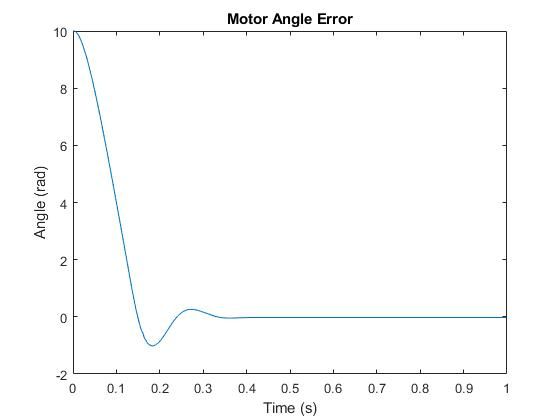
\includegraphics[width=0.8\textwidth]{./figures/lab4_fig7-part4-3-3-error-rc5.jpg}
        \caption{System 1 Response to Constant Input}
        \label{fig:system1_constant}
\end{figure}

\begin{figure}[H]
        \centering
        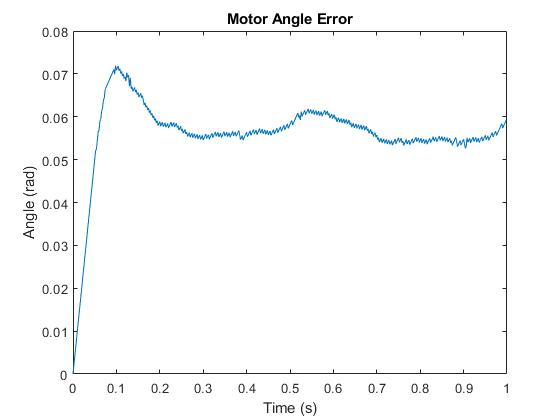
\includegraphics[width=0.8\textwidth]{./figures/lab4_fig8-part4-3-3-error-rc5-linear.jpg}
        \caption{System 1 Response to Linear Input}
        \label{fig:system1_linear}
\end{figure}

\begin{figure}[H]
        \centering
        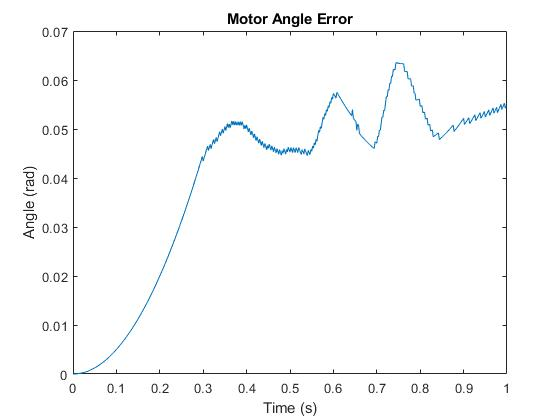
\includegraphics[width=0.8\textwidth]{./figures/lab4_fig9-part4-3-3-error-rc5-quadratic.jpg}
        \caption{System 1 Response to Quadratic Input}
        \label{fig:system1_quadratic}
\end{figure}

\begin{figure}[H]
        \centering
        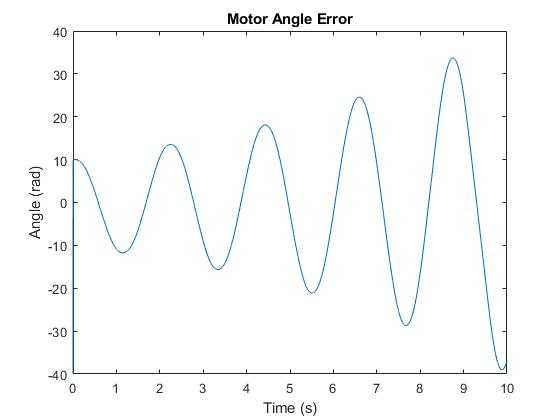
\includegraphics[width=0.8\textwidth]{./figures/lab4_fig10-part4-3-3-error-rc-I=1-constant.jpg}
        \caption{System 2 Response to Constant Input}
        \label{fig:system2_constant}
\end{figure}

\begin{figure}[H]
        \centering
        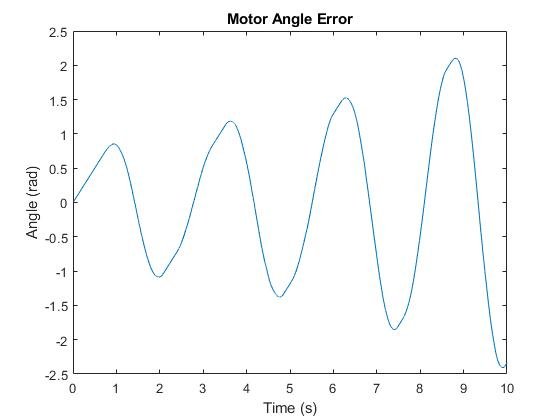
\includegraphics[width=0.8\textwidth]{./figures/lab4_fig11-part4-3-3-error-rc-I=1-linear.jpg}
        \caption{System 2 Response to Linear Input}
        \label{fig:system2_linear}
\end{figure}

\begin{figure}[H]
        \centering
        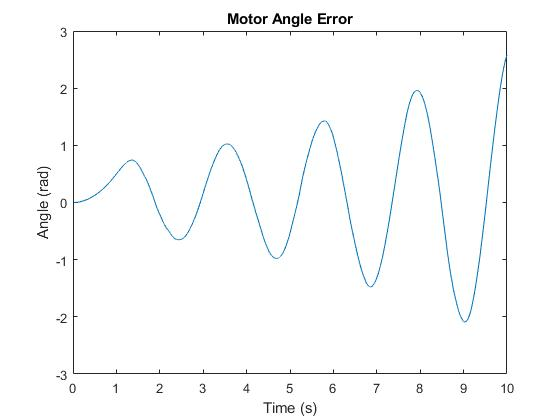
\includegraphics[width=0.8\textwidth]{./figures/lab4_fig12-part4-3-3-error-rc-I=1-quadratic.jpg}
        \caption{System 2 Response to Quadratic Input}
        \label{fig:system2_quadratic}
\end{figure}

\begin{figure}[H]
        \centering
        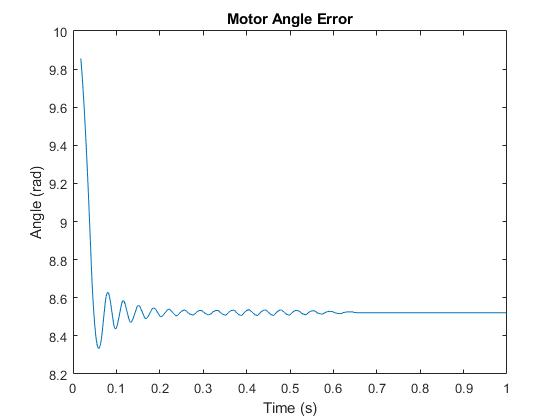
\includegraphics[width=0.8\textwidth]{./figures/lab4_fig13-part4-3-3-error-rc-D=1-constant.jpg}
        \caption{System 3 Response to Constant Input}
        \label{fig:system3_constant}
\end{figure}

\begin{figure}[H]
        \centering
        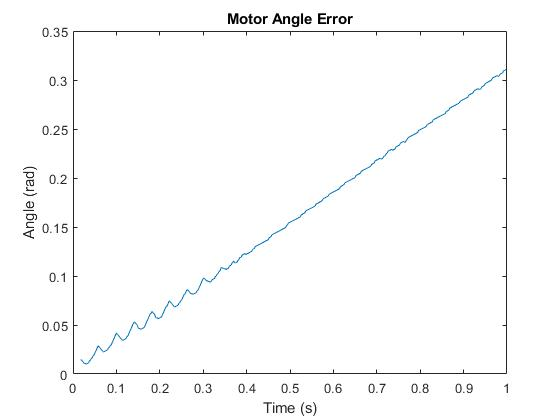
\includegraphics[width=0.8\textwidth]{./figures/lab4_fig14-part4-3-3-error-rc-D=1-linear.jpg}
        \caption{System 3 Response to Linear Input}
        \label{fig:system3_linear}
\end{figure}

\begin{figure}[H]
        \centering
        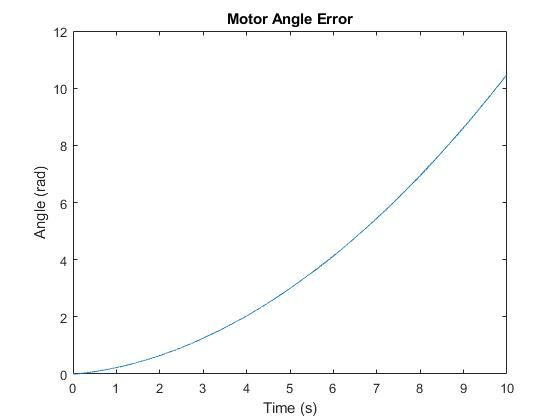
\includegraphics[width=0.8\textwidth]{./figures/lab4_fig15-part4-3-3-error-rc-D=1-quadratic.jpg}
        \caption{System 3 Response to Quadratic Input}
        \label{fig:system3_quadratic}
\end{figure}
